% pdflatex -shell-escape template_rapport.tex

\documentclass[a4paper,oneside]{article}

\usepackage[frenchb]{babel}
\usepackage[utf8]{inputenc}
%\usepackage[T1]{fontenc}
\usepackage{graphicx}
\usepackage{amssymb} 
\usepackage{amsmath}
\usepackage{hyperref}
\usepackage{fullpage}
\usepackage{titlesec}
\usepackage{fancyhdr}
\usepackage{nopageno}

%%%%%%%%%%%%%%%%%%%%%%%%%

\title{Rapport du projet Machin}
\author{}
\date{}

\makeatletter
\pagestyle{fancy}
\fancyhf{}
\fancyhead[L]{}
\fancyhead[C]{}
\fancyhead[R]{}
\renewcommand{\headrulewidth}{0pt}
\fancyfoot[L]{\@title}
\fancyfoot[C]{}
\fancyfoot[R]{page \thepage / \pageref{myLastPage}}
\renewcommand{\footrulewidth}{0.4pt}

%%%%%%%%%%%%%%%%%%%%%%%%%

\begin{document}

%%%%%%%%%%%%%%%%%%%%%%%%%

\thispagestyle{empty}

\Large
ULCO - L3 Informatique

\vfill 

\Huge
\begin{center}
\@title
\end{center}

\normalsize

\vfill 

\paragraph{Étudiants : }

\paragraph{Encadrant : }

\paragraph{Date de début : }

\paragraph{Date de fin : }

\paragraph{Objet du projet : }

~

\vfill 

\noindent\rule{\linewidth}{0.5pt}

\tableofcontents

~\\
\noindent\rule{\linewidth}{0.5pt}

\clearpage

%%%%%%%%%%%%%%%%%%%%%%%%%

\section{Présentation du projet}

2 pages max 

\subsection{Analyse de la demande}

Contexte…

Besoins, priorités…


\subsection{Spécifications}

\begin{enumerate}
    \item …
    \item …
\end{enumerate}

\clearpage

%%%%%%%%%%%%%%%%%%%%%%%%%


\section{Réalisation}
Description et justification des choix techniques. 

Des schémas commentés mais pas de code ni de blabla inutile.

4 pages max 

\subsection{Présentation }
Le logiciel implémenté permet de charger un fichier de données (spécification 13) et d'afficher ces données en même temps dans un terminal et dans une fenêtre graphique (spécification 37).

\begin{center}
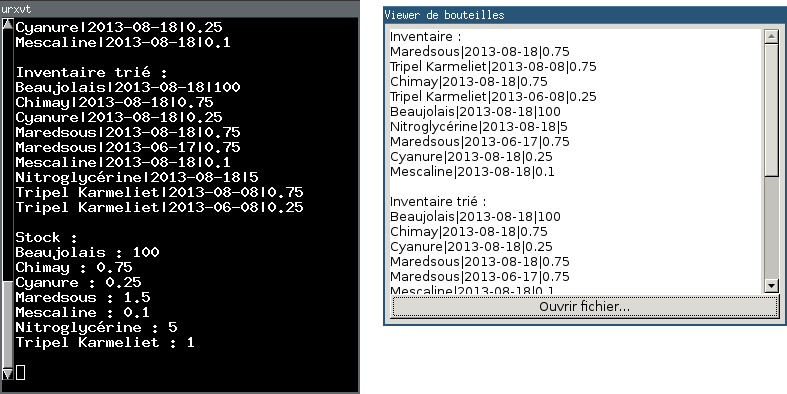
\includegraphics[width=9cm]{capture_ecran.png}
\end{center}

\paragraph{}
De plus, pour répondre à la spécification … on a implémenté …

\paragraph{}
Enfin, comme convenu dans le cahier des charges, le logiciel fonctionne sur l'environnement … avec les bibliothèques …


\subsection{Architecture générale}
On a utilisé un MVC parce que …

\begin{center}
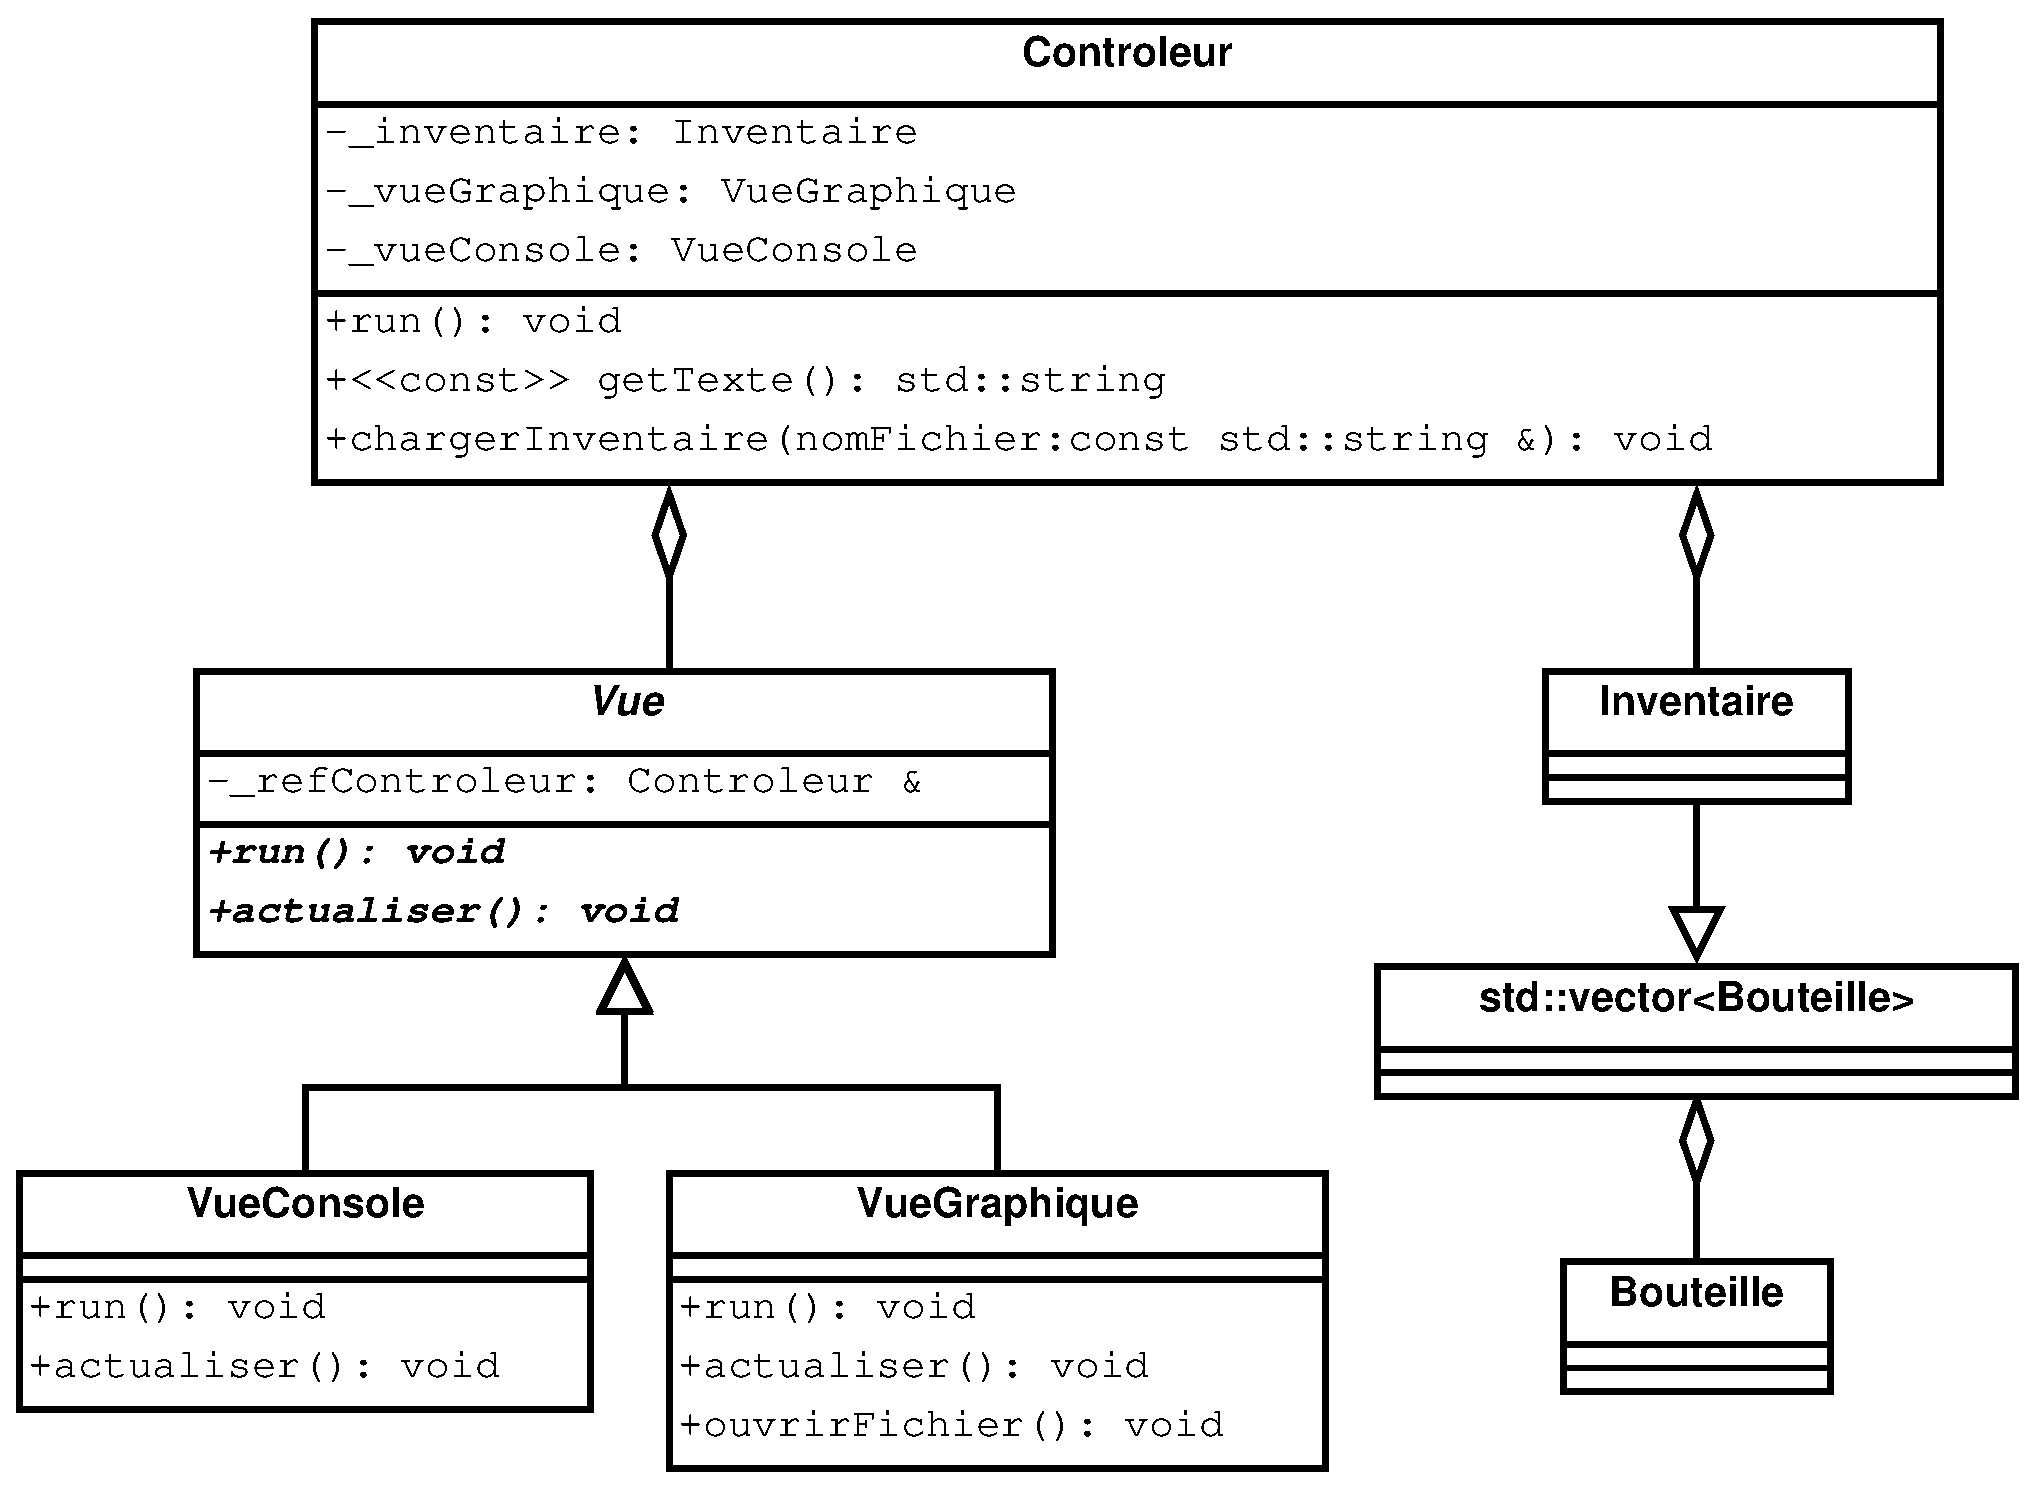
\includegraphics[width=10cm]{architecture_generale.eps}
\end{center}


\subsection{Gestion de ceci}

\subsection{Gestion de cela}

\clearpage

%%%%%%%%%%%%%%%%%%%%%%%%%


\section{Bilan}

2 pages max 

\subsection{Déroulement du projet}

Différences par rapport aux prévisions (conception, planification…), problèmes rencontrés, solutions adoptées.


\subsection{Réalisation des objectifs }

\begin{tabular}{| l | c |}
\hline
fonctionnalité & réalisation \\
\hline
\hline
fonctionnalité 1 & complète \\
\hline
fonctionnalité 2 & partielle \\
\hline
fonctionnalité 3 & non \\
\hline
\end{tabular}

\paragraph{}
Pour la fonctionnalité 2, il y a … Par rapport aux spécifications demandées, il manque …


\subsection{Conclusion pour les projets futurs}

Ce qui a bien marché, les erreurs à ne plus commettre.



%%%%%%%%%%%%%%%%%%%%%%%%%

\label{myLastPage}

\end{document}

%%%%%%%%%%%%%%%%%%%%%%%%%

